%\documentclass[mathserif]{beamer}
\documentclass[handout]{beamer}
%\usetheme{Goettingen}
%\usetheme{Warsaw}
\usetheme{Singapore}



%\usetheme{Frankfurt}
%\usetheme{Copenhagen}
%\usetheme{Szeged}
%\usetheme{Montpellier}
%\usetheme{CambridgeUS}
%\usecolortheme{}
%\setbeamercovered{transparent}
\usepackage[english, activeacute]{babel}
\usepackage[utf8]{inputenc}
\usepackage{amsmath, amssymb}
\usepackage{dsfont}
\usepackage{graphics}
\usepackage{cases}
\usepackage{graphicx}
\usepackage{pgf}
\usepackage{epsfig}
\usepackage{amssymb}
\usepackage{multirow}	
\usepackage{amstext}
\usepackage{algorithm2e}
\usepackage{amsmath}
\usepackage{epic}
\usepackage{epsfig}
\usepackage{fontenc}
\usepackage{framed,color}
\usepackage{palatino, url, multicol}
%\algsetup{indent=2em}
\newcommand{\factorial}{\ensuremath{\mbox{\sc Factorial}}}
\newcommand{\BIGOP}[1]{\mathop{\mathchoice%
{\raise-0.22em\hbox{\huge $#1$}}%
{\raise-0.05em\hbox{\Large $#1$}}{\hbox{\large $#1$}}{#1}}}
\newcommand{\bigtimes}{\BIGOP{\times}}
\vspace{-0.5cm}
\title{Acquiring and Exploiting Lexical Knowledge for Twitter Sentiment Analysis}
\vspace{-0.5cm}
\author[Felipe Bravo Márquez]{\footnotesize
%\author{\footnotesize  
 \textcolor[rgb]{0.00,0.00,1.00}{Felipe Bravo-Marquez} \\ Chief Supervisor: Bernhard Pfahringer \\  Supervisor: Eibe Frank} 
  
 
%\vspace{-0.3cm}
\institute{Department of Computer Science, University of Waikato }

\titlegraphic{
\includegraphics[scale=0.3]{pics/logo.pdf}}



\date{17 July, 2017}

\begin{document}
\begin{frame}
\titlepage


\end{frame}

\section{Introduction}


\begin{frame}{Message-level Polarity Classification (MPC)}
\begin{scriptsize}
  \begin{enumerate}
   \item Automatically classify a tweet to classes \textcolor[rgb]{0.00,0.00,1.00}{\textbf{positive}}, \textcolor[rgb]{1.00,0.00,0.00}{\textbf{negative}}, or \textcolor[rgb]{0.00,1.00,0.00}{\textbf{neutral}}. 
   
     \begin{figure}[h]
        	
\includegraphics[scale = 0.15]{pics/sent.png}
        \end{figure}
   \item Challenge: Tweets use a unique \textbf{informal dialect} including many abbreviations, acronyms, misspelled words, hashtags, and emoticons, e.g., \textbf{lol}, \textbf{omg}, \textbf{hahaha}, \textbf{\#hatemonday}, \textbf{\#SweetAsBro}, \textbf{\#yeahnah}, \textbf{:)} .
   \item State-of-the-art solutions use \textbf{supervised} machine learning models trained from \textbf{manually} annotated examples \cite{NRCJAIR14}.
   \item \textbf{Label sparsity problem (LS)}: manual annotation is \textbf{labour-intensive} and \textbf{time-consuming}. 
  \end{enumerate} 
\end{scriptsize}

\end{frame}



\begin{frame}{Research Problem}

This thesis addresses the label sparsity problem for Twitter sentiment classification by automatically building \textbf{two type of resources}. 
\begin{enumerate}
 \item \textbf{Twitter-specific opinion lexicons}: we develop machine learning models to induce polarity lexicons from tweets. 
 \item  \textbf{Synthetically labelled tweets}: we develop distant supervision methods based on \textbf{lexical knowledge} (we go beyond emoticons). 
 \end{enumerate}

\end{frame}


\section{Polarity Lexicon Induction}


\begin{frame}{Word-sentiment Associations for Polarity Lexicon Induction}
\begin{figure}[htb]
	\centering
	 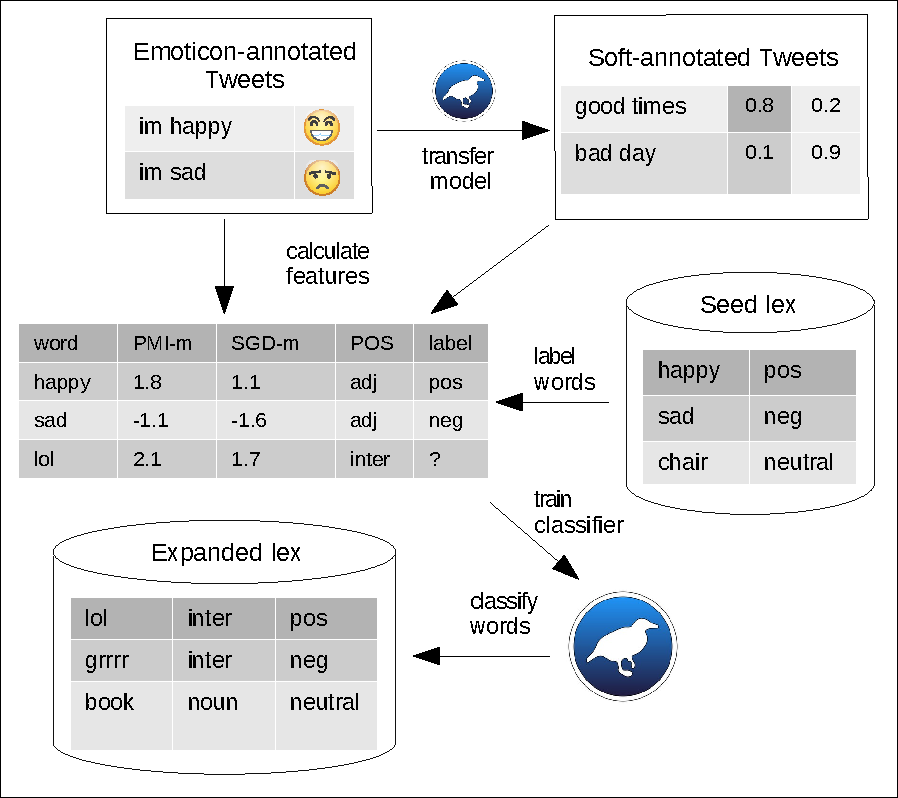
\includegraphics[scale=0.5]{pics/diagramcrop.pdf}
	\label{fig:sosgd}
\end{figure}
\end{frame}



\begin{frame}{Word-level Classification Results using RBF SVMs}
\footnotesize
\begin{table}[!htb]
\begin{center}
\begin{tabular}{l|l|l}
\hline \hline
\multicolumn{ 3}{c}{Weighted AUC } \\ \hline \hline
Dataset & PMI-SO & ALL FEATURES \\ \hline
ED.EM & 0.62 $\pm$ 0.02 &  \textbf{0.65 $\pm$ 0.02} $+$ \\  
STS & 0.64 $\pm$ 0.02 & \textbf{0.66 $\pm$ 0.01} $+$   \\ 
%ED.T07 & 0.62 $\pm$ 0.02 & \textbf{0.65 $\pm$ 0.02} $+$   \\ 
ED.SL &  0.63 $\pm$ 0.02 & \textbf{0.65  $\pm$  0.02} $+$ \\ \hline 
\end{tabular}
\end{center}
\caption{World-level classification performance.} 
\label{tab:classres}
\end{table}
\end{frame}







\begin{frame}{Tweet-centroid Model for Lexicon Induction}

\begin{figure}[htb]
	\centering
	 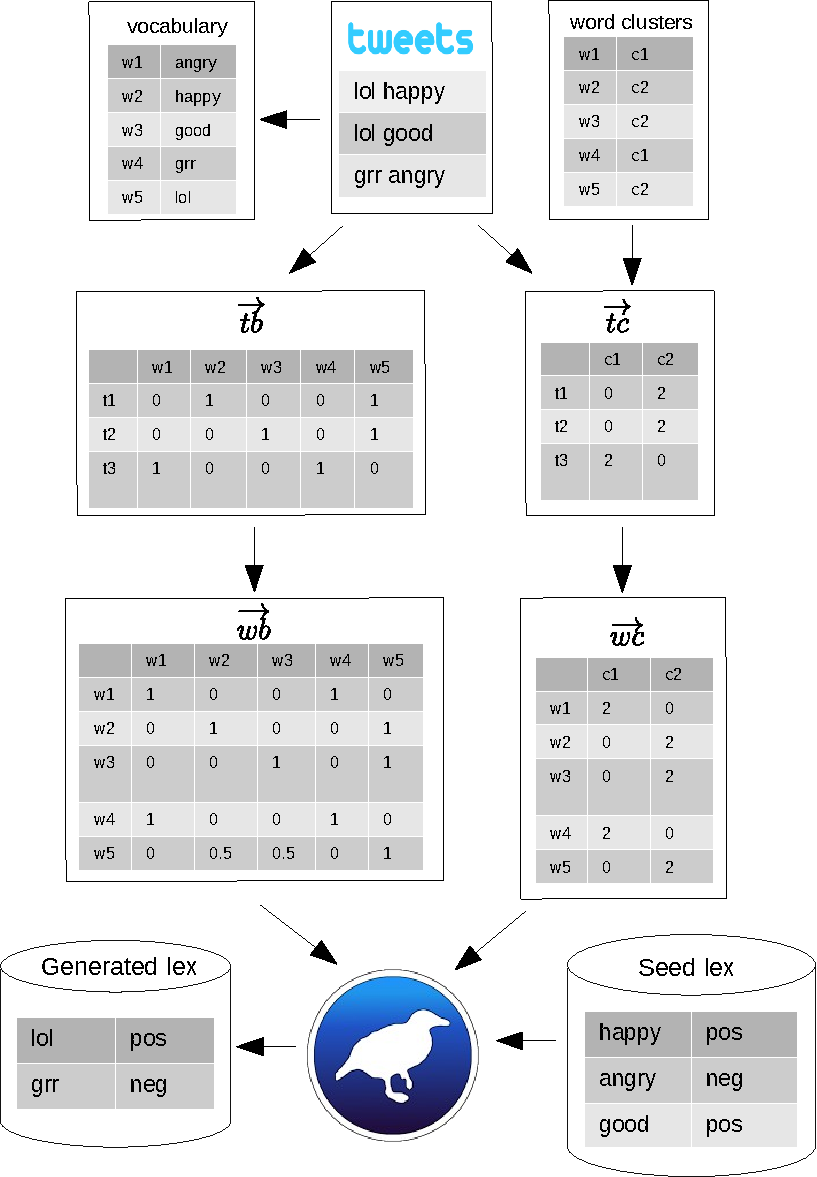
\includegraphics[scale=0.4]{sigirmodel.pdf}
\end{figure}



\end{frame}




\begin{frame}{Message-level classification performance}
\begin{scriptsize}
 \begin{table}[htbp]
\scriptsize
\begin{center}
\begin{tabular}{l|c|c}
\hline \hline
\multicolumn{ 3}{c}{AUC} \\ \hline \hline
Dataset & Seed Lexicon  & TCM Lexicon \\ \hline
Sanders & 0.78 $\pm$ 0.04 & \textbf{0.83 $\pm$ 0.04} $+$ \\ 
6-human & 0.79 $\pm$ 0.03 & \textbf{0.83 $\pm$ 0.02} $+$ \\ 
SemEval & 0.78 $\pm$ 0.02 & \textbf{0.84 $\pm$ 0.02} $+$ \\ \hline
\end{tabular}
\end{center}
\end{table}
\end{scriptsize}
\end{frame}


\begin{frame}{Multi-Label Classification of Emotions with TCM}
\begin{scriptsize}

\begin{figure}[htbp]
\begin{center}
\scalebox{0.7}{
\begin{tabular}{cccc}
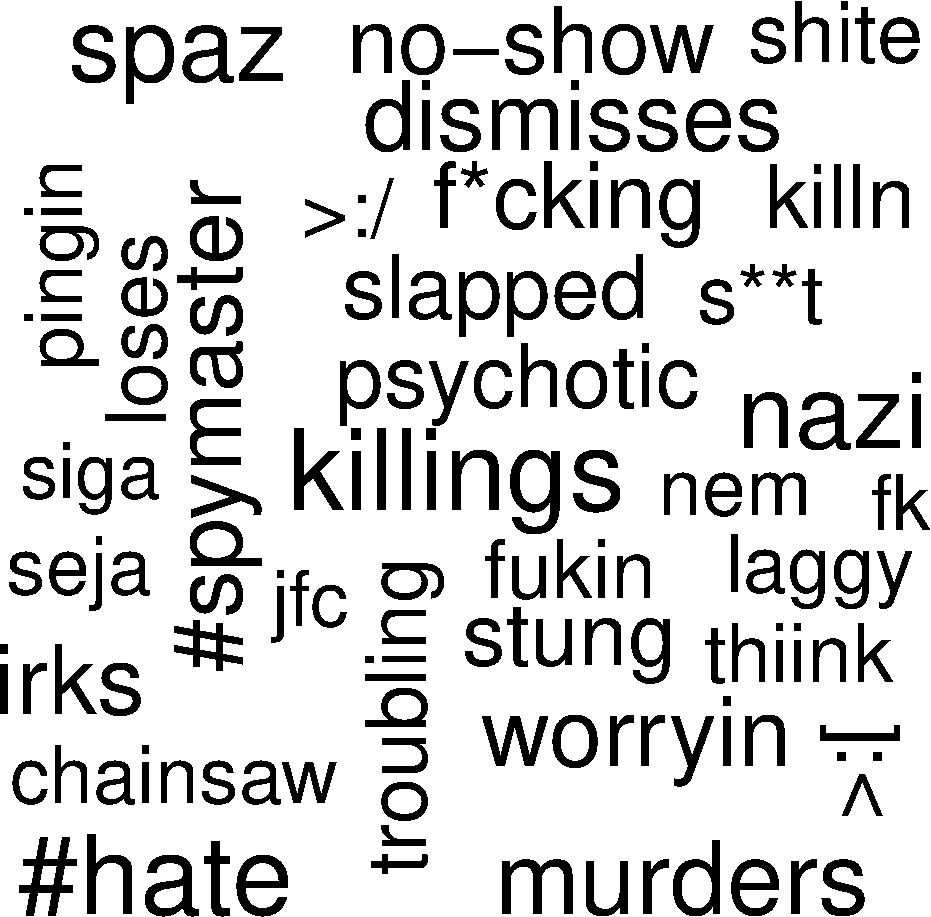
\includegraphics[scale=0.2]{pics/anger.pdf} & 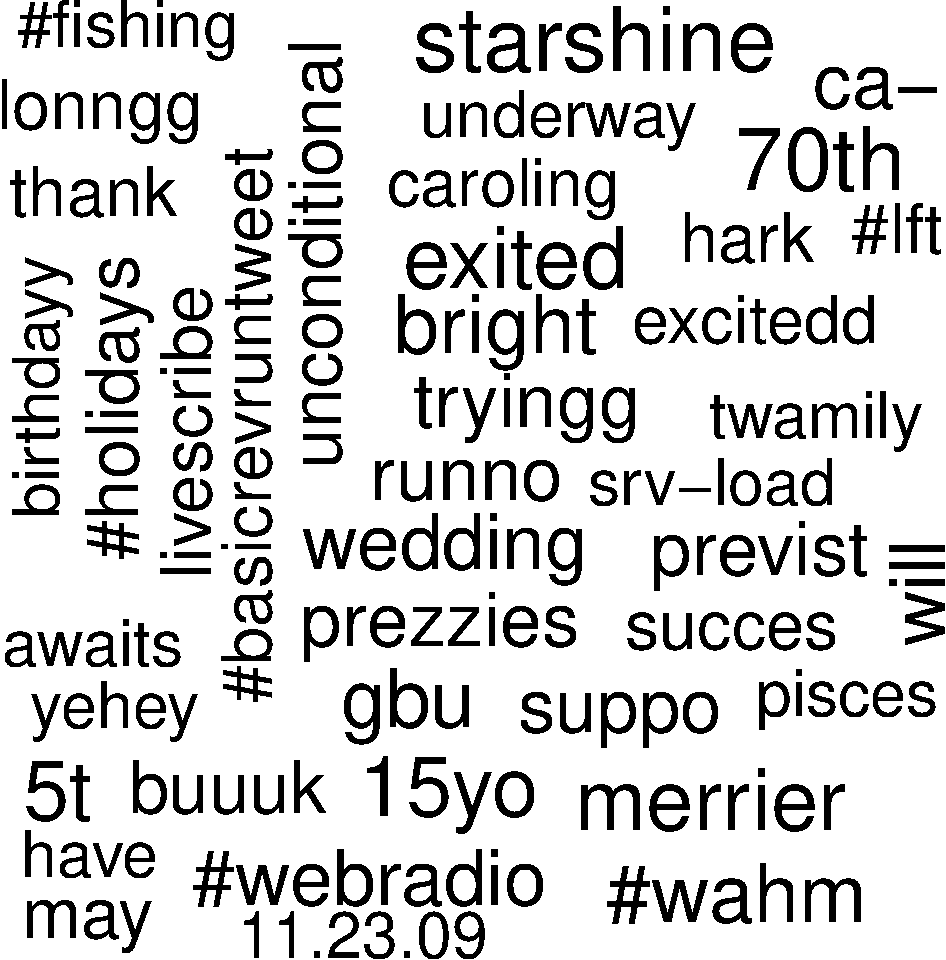
\includegraphics[scale=0.2]{pics/ant.pdf} & 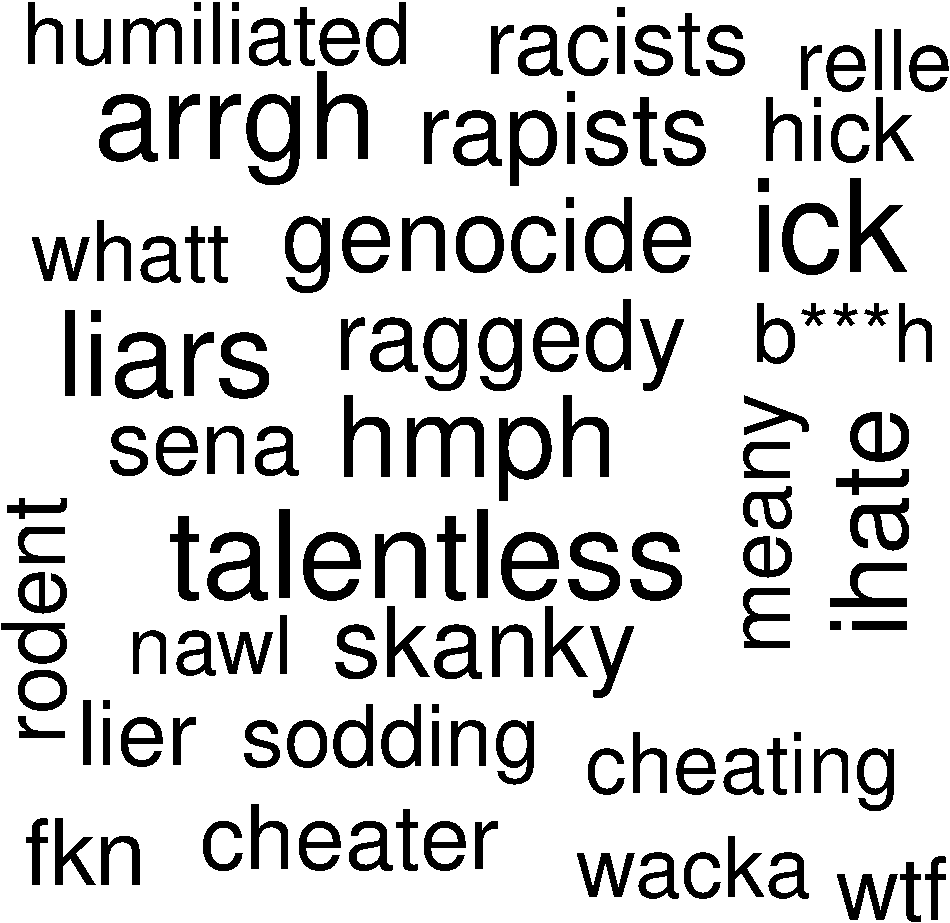
\includegraphics[scale=0.2]{pics/disg.pdf} & 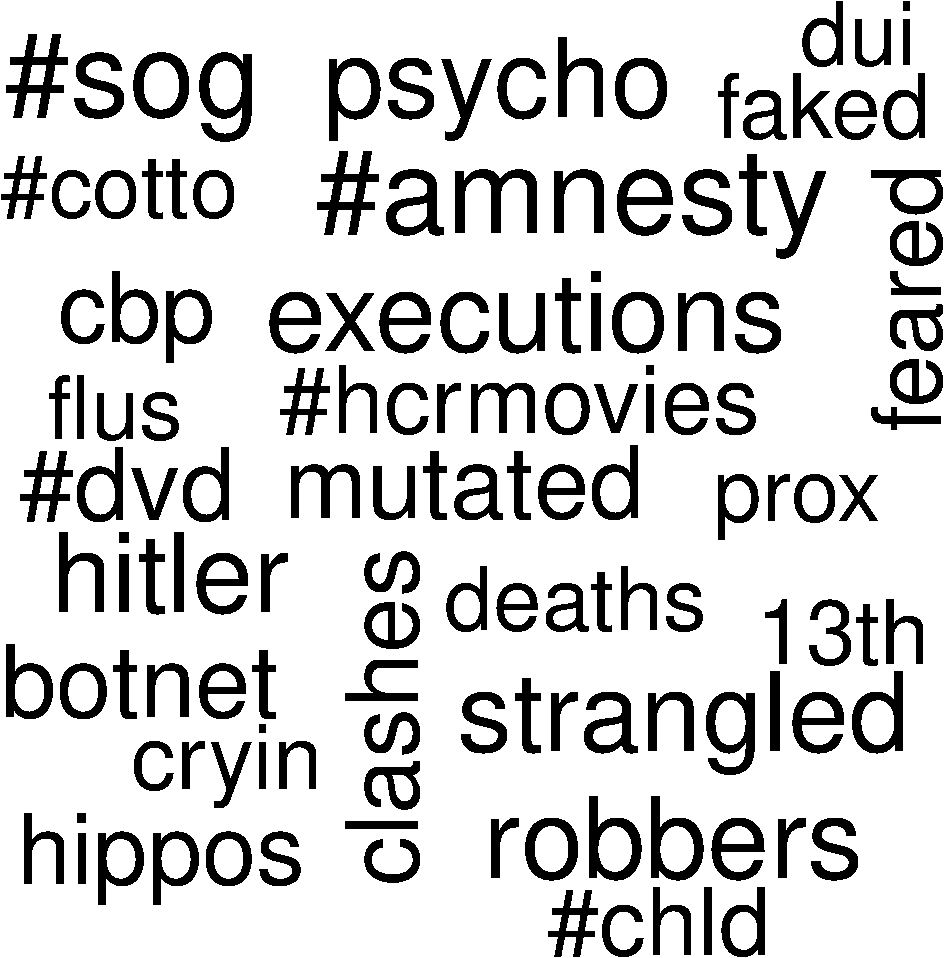
\includegraphics[scale=0.2]{pics/fear.pdf} \\
anger & anticipation & disgust & fear\\[1mm] 
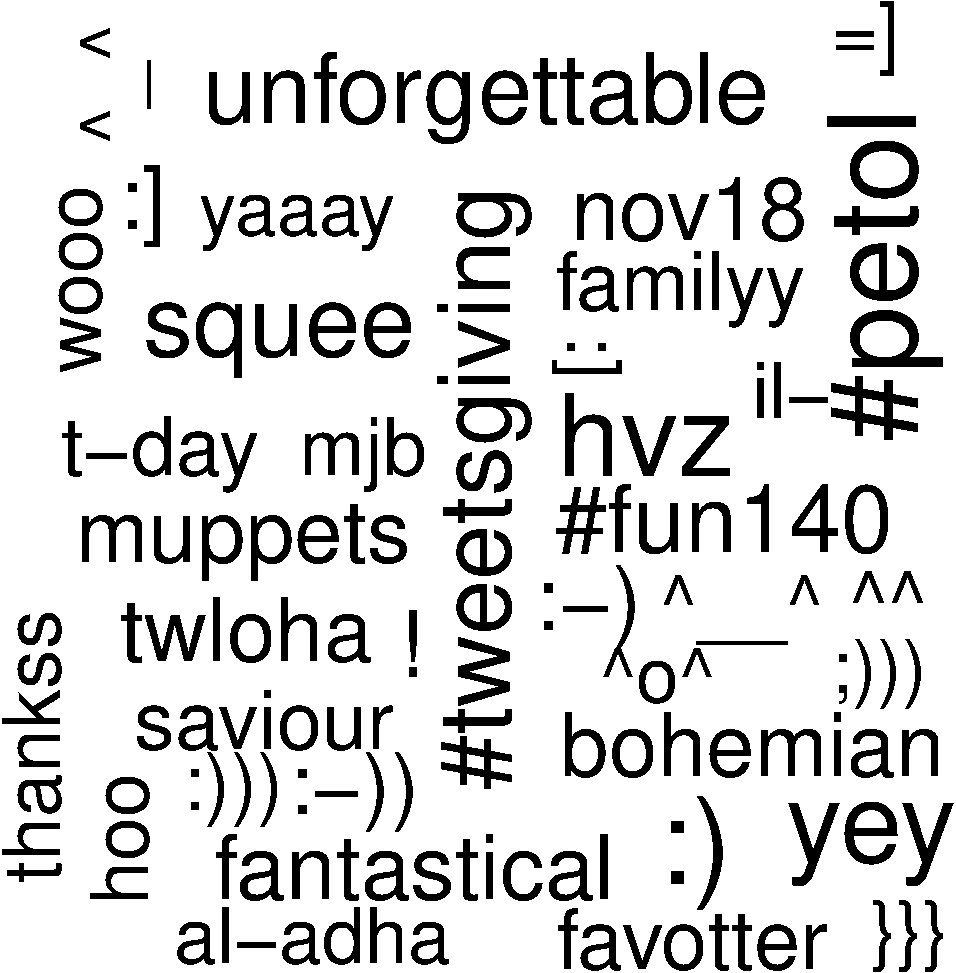
\includegraphics[scale=0.2]{pics/joy.pdf} & 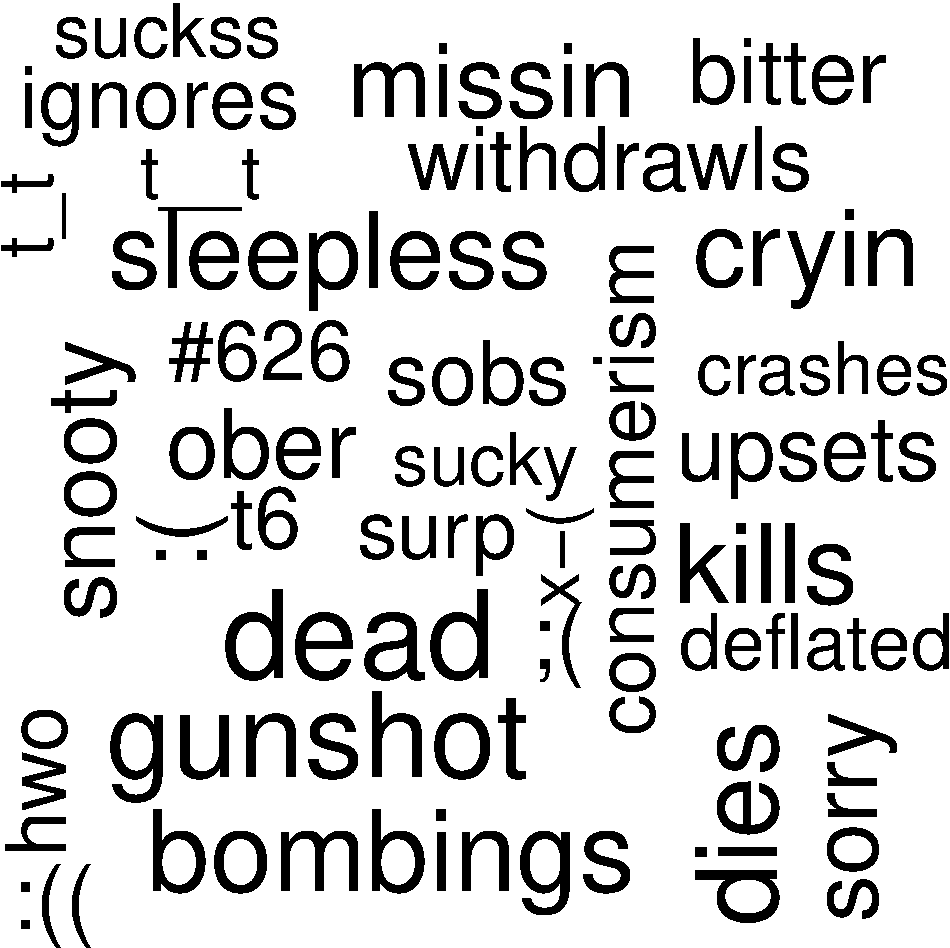
\includegraphics[scale=0.2]{pics/sadness.pdf} & 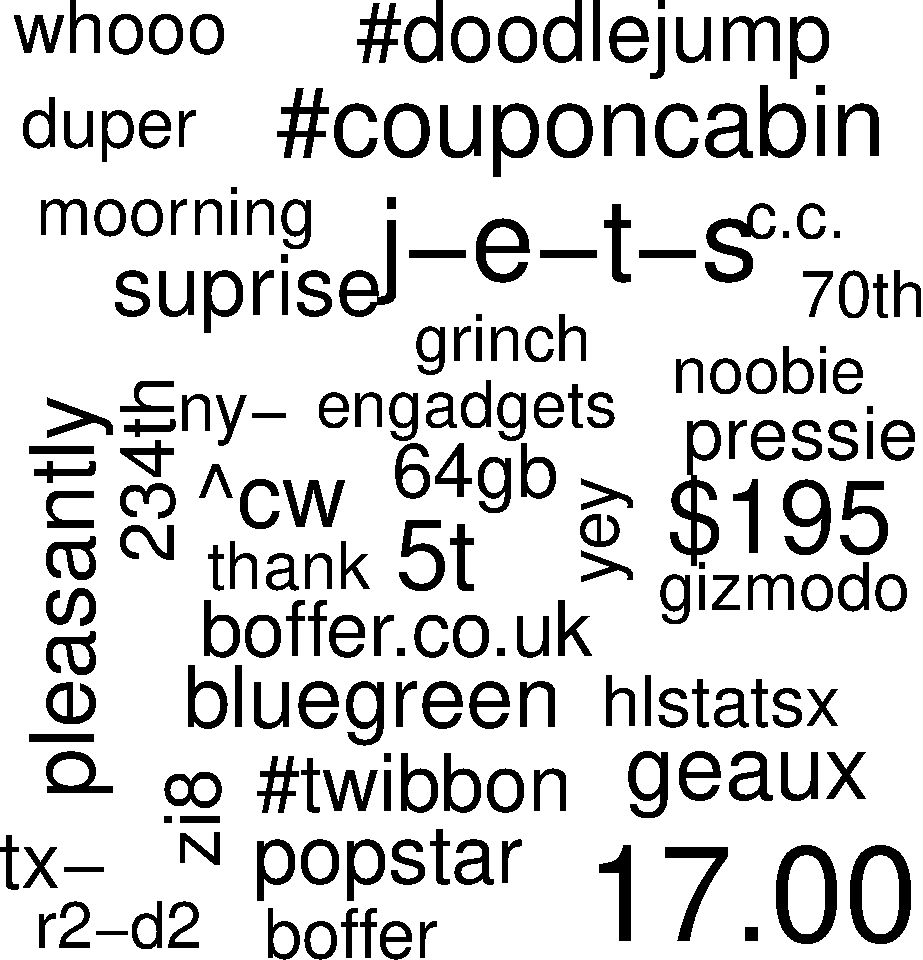
\includegraphics[scale=0.2]{pics/surprise.pdf} & 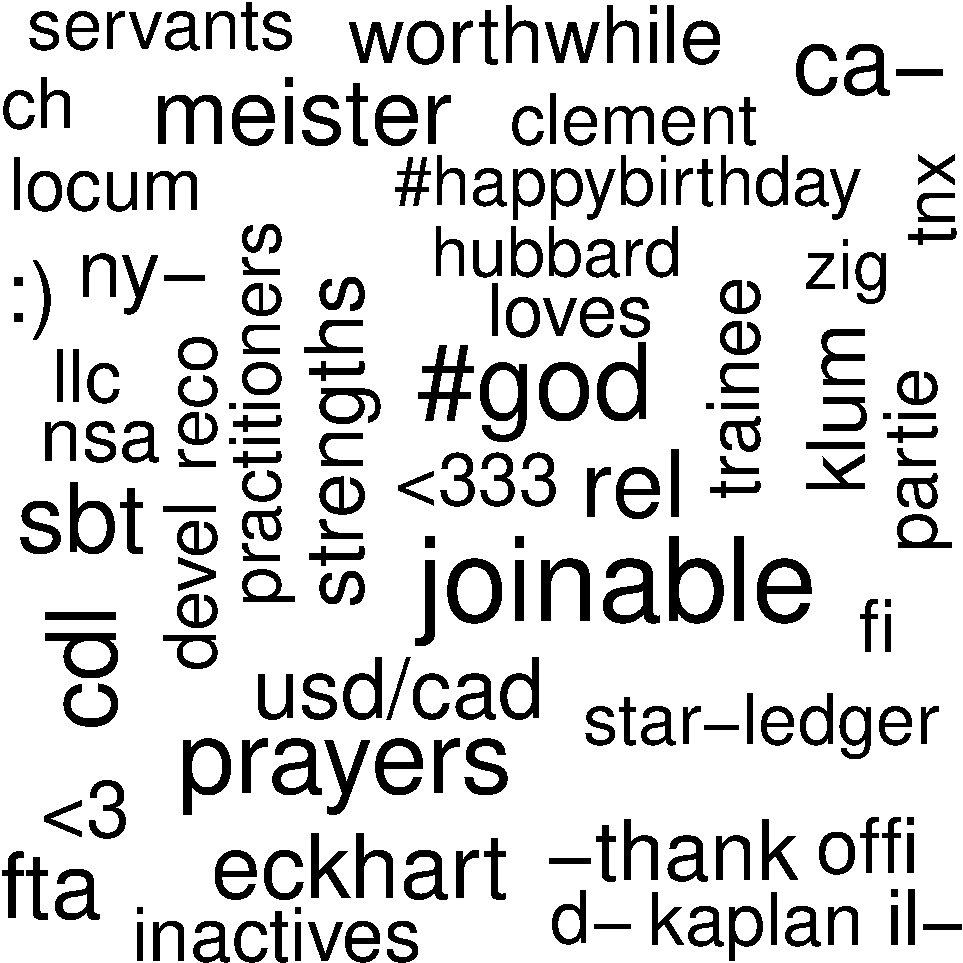
\includegraphics[scale=0.2]{pics/trust.pdf} \\
joy & sadness & surprise & trust\\
\end{tabular}}
\end{center}
\end{figure}

\end{scriptsize}
\end{frame}

\section{Distant Supervision}

\begin{frame}{Transfer Learning with Tweet Centroids}

\begin{figure}[htb]
	\centering
	 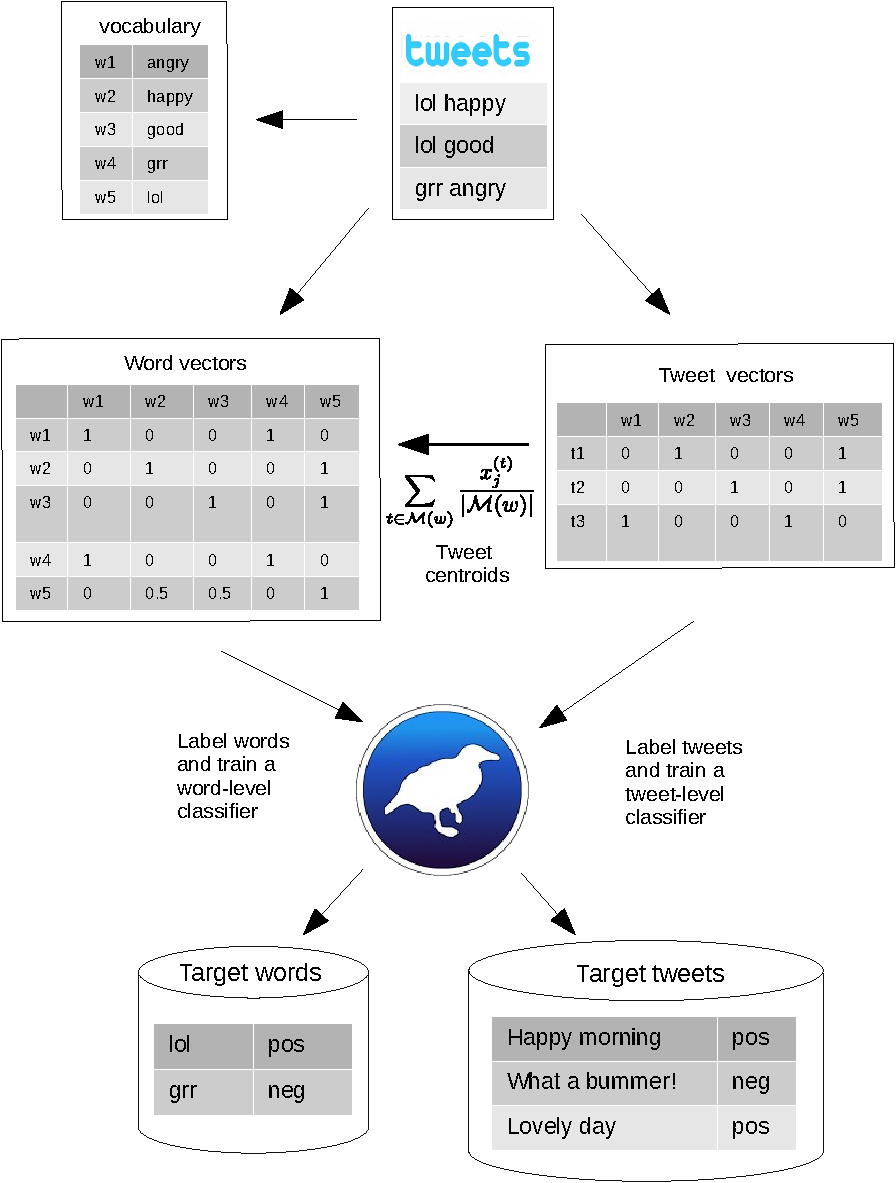
\includegraphics[scale=0.4]{pics/tweetsToWords.pdf}
\end{figure}



\end{frame}


\begin{frame}{Partitioned TCM}
\begin{scriptsize}
\begin{itemize}
\item We propose a modification of TCM for \textbf{increasing} the number of labelled instances it produces. 
\item  The word-tweet set $\mathcal{M}(w)$ is \textbf{partitioned} into smaller disjoint subsets $\mathcal{M}(w)_1, \dots \mathcal{M}(w)_z$ of a fixed size determined by $p$. 
\item We calculate one tweet centroid vector $\overrightarrow{w}$ for \textbf{each partition} labelled according to $\mathcal{L}$.
\end{itemize}
\end{scriptsize}
\end{frame}



\begin{frame}{TCM for MPC}

\begin{table}[htbp]
\begin{center}
\scalebox{0.8}{
\begin{tabular}{l|ll@{\hspace{0.1cm}}l@{\hspace{0.1cm}}|ll@{\hspace{0.1cm}}l@{\hspace{0.1cm}}|ll@{\hspace{0.1cm}}l@{\hspace{0.1cm}}}
\hline
 & \multicolumn{3}{c|}{6HumanCoded} & \multicolumn{3}{c|}{Sanders} & \multicolumn{3}{c}{SemEval} \\ \hline
EAA & 0.805 $\pm$ 0.005 & = & - & 0.800 $\pm$ 0.017 & = & +& 0.802  $\pm$ 0.006 & = & - \\ 
LAA & 0.809 $\pm$ 0.001 & + & = & 0.778 $\pm$ 0.002 & - & = & 0.814  $\pm$ 0.000 &+ & =\\ \hline
TCM & 0.776 $\pm$ 0.004 &-&-& 0.682 $\pm$ 0.024 &-&-& 0.779  $\pm$ 0.008 &-&-\\ 
TCM ($p$=5) & 0.834 $\pm$ 0.002 & + & +& 0.807 $\pm$ 0.008 &= & +& 0.833  $\pm$ 0.002 &+&+ \\ 
TCM ($p$=10) & 0.845 $\pm$ 0.003 & + & +& \textbf{0.817} $\pm$ 0.006 &+ & +& 0.841  $\pm$ 0.002 &+ & +\\ 
TCM ($p$=20) & \textbf{0.850} $\pm$ 0.003 &+ & +& 0.815 $\pm$ 0.011 &+ & +& \textbf{0.844}  $\pm$ 0.003 & + & +\\ 
TCM ($p$=50) & 0.844 $\pm$ 0.004 & + & +& 0.785 $\pm$ 0.010 & - & +& 0.836  $\pm$ 0.004 & + & +\\ 
TCM ($p$=100) & 0.829 $\pm$ 0.003 & + & +& 0.752 $\pm$ 0.019 & - & -& 0.821  $\pm$ 0.004 & + & +\\ \hline
\end{tabular}}
\end{center}
\caption{Message-level Polarity Classification Results. Best results per column are given in bold.}
\label{tab:messclas}
\end{table}
\end{frame}




\begin{frame}{Annotate-Sample-Average (ASA)}
\begin{scriptsize}
 \begin{itemize}
  \item What if we average random tweets containing \textbf{different words} with the same polarity?
 \item What if we can define the \textbf{number of instances} to generate?
 \item This could be useful for creating \textbf{compact and balanced} training datasets. 
 \end{itemize}
 
 
 \begin{block}{ASA algorithm}
\begin{enumerate}
 \item \textbf{Annotation}: every time a word from $\mathcal{L}$  is found, the  tweet is added to sets \textbf{posT} or \textbf{negT} (depending on the polarity).
 \item \textbf{Sample}: randomly sample with replacement $a$ tweets from either \textbf{posT} or \textbf{negT} for each generated instance. 
 \item \textbf{Averaging}: average and label sampled feature vectors.
\end{enumerate}
\end{block}
 
  
\end{scriptsize} 
\end{frame}


\begin{frame}{ASA results}
\begin{table}[htb]
\begin{center}
\scalebox{0.6}{
\begin{tabular}{l|ll@{\hspace{0.1cm}}l@{\hspace{0.1cm}}l@{\hspace{0.1cm}}l@{\hspace{0.1cm}}|ll@{\hspace{0.1cm}}l@{\hspace{0.1cm}}l@{\hspace{0.1cm}}l@{\hspace{0.1cm}}|ll@{\hspace{0.1cm}}l@{\hspace{0.1cm}}l@{\hspace{0.1cm}}l@{\hspace{0.1cm}}l@{\hspace{0.1cm}}l@{\hspace{0.1cm}}l@{\hspace{0.1cm}}l@{\hspace{0.1cm}}}
\hline
 & \multicolumn{ 5}{c|}{6HumanCoded} & \multicolumn{5}{c|}{Sanders} & \multicolumn{5}{c}{SemEval} \\ \hline
EAA\_U & 0.805 $\pm$ 0.005 & = & = & - & - & 0.800 $\pm$ 0.017 & = & = & + & + & 0.802 $\pm$ 0.006 & = & + & - & - \\ 
EAA\_B &  0.809 $\pm$ 0.001 & = & = & = & = & 0.795 $\pm$ 0.016 & = & = & + & + & 0.798 $\pm$ 0.007 & - & = & - & - \\ 
LAA\_U & 0.809 $\pm$ 0.001 & + & = & = & = & 0.778 $\pm$ 0.002 & - & - & = & = & 0.814 $\pm$ 0.000 & + & + & = & = \\ 
LAA\_B & 0.809 $\pm$ 0.001 & + & = & = & = & 0.778 $\pm$ 0.003 & - & - & = & = & 0.813 $\pm$ 0.001 & + & + & = & = \\ \hline
ASA ($a=1$, $m=F$) & 0.793 $\pm$ 0.005 & - & - & - & -  & 0.762 $\pm$ 0.016 & - & - & - & -  & 0.787 $\pm$ 0.007 & - & - & - & -  \\ 
ASA ($a=5$, $m=F$)  & 0.837 $\pm$ 0.004 & + & + & + & +  & 0.807 $\pm$ 0.010 & = & = & + & +  & 0.833 $\pm$ 0.003 & + & + & + & +  \\ 
ASA ($a=10$, $m=F$) & \textbf{0.845} $\pm$ 0.001 & + & + & + & +  & \textbf{0.812} $\pm$ 0.015 & + & + & + & +  & \textbf{0.840} $\pm$ 0.003 & + & + & + & +  \\ 
ASA ($a=50$, $m=F$) & 0.815 $\pm$ 0.003 & + & + & + & +  & 0.759 $\pm$ 0.006 & - & - & - & -  & 0.810 $\pm$ 0.004 & + & + & - & - \\ 
ASA ($a=100$, $m=F$)  & 0.781 $\pm$ 0.003 & - & - & - & -  & 0.720 $\pm$ 0.007 & - & - & - & -  & 0.779 $\pm$ 0.004 & - & - & - & -  \\ 
ASA ($a=500$, $m=F$)  & 0.723 $\pm$ 0.002 & - & - & - & -  & 0.670 $\pm$ 0.008 & - & - & - & -  & 0.729 $\pm$ 0.005 & - & - & - & -  \\ 
ASA ($a=1000$, $m=F$) & 0.712 $\pm$ 0.002 & - & - & - & -  & 0.665 $\pm$ 0.007 & - & - & - & -  & 0.721 $\pm$ 0.005 & - & - & - & -  \\ 
\end{tabular}}
\end{center}
\caption{AUC measure for different distant supervision models. Best results per column are given in bold. }
\label{tab:resA}
\end{table} 
 
 
\end{frame}



\section{Conclusions}

\begin{frame}{Conclusions}
\begin{scriptsize}
\begin{itemize}
\item Twitter-specific polarity lexicons and lexicon-based distant supervision methods can successfully tackle the polarity classification of tweets when labels are \textbf{scarce}.

\item We proposed two methods (Word Sentiment Associations and TCM) for building Twitter-specific \textbf{opinion lexicons} (acquisition of lexical knowledge).

\item These methods could be used to create \textbf{domain-specific} lexicons.
\item They could also be used to study the \textbf{dynamics} of opinion-words.
\item Future work: try \textbf{non-linear representations} on TCM (Auto-Encoders or RBM).

\end{itemize}
\end{scriptsize}

\end{frame}



\begin{frame}{Conclusions}
\begin{scriptsize}
\begin{itemize}
\item  We proposed two \textbf{distant supervision methods} (TCM and ASA) that outperformed LAA and EAA for MPC.

\item TCM is a \textbf{unified model} for message-level and word-level sentiment classification.


\item Future work: subjectivity, emotions, handle negations, non-linear representations and deep networks. 
\end{itemize}
\end{scriptsize}

\end{frame}



\begin{frame}
\frametitle{Questions?}
%\vspace{1.5cm}
\begin{center}\LARGE Thanks for your Attention!\\  \end{center}

\begin{columns}
\begin{column}{0.55\textwidth}
\begin{block}{Acknowledgements}
\begin{itemize}\tiny
	\item University of Waikato Doctoral Scholarship
	\item Machine Learning Group at the University of Waikato
	
\end{itemize}
\end{block}
\end{column}
\begin{column}{0.45\textwidth}
\vspace{1.5cm}

\begin{figure}[h!]
	\centering
	
\includegraphics[scale=0.3]{pics/logo.pdf}
\end{figure}
\end{column}
\end{columns}

\end{frame}

\begin{frame}[allowframebreaks]\scriptsize
\frametitle{References}
\bibliography{../bio}
\bibliographystyle{apalike}
%\bibliographystyle{flexbib}
\end{frame}  


%%%%%%%%%%%%%%%%%%%%%%%%%%%

\end{document}
